\documentclass[11pt]{article}

\usepackage{amsfonts}
\usepackage{amsmath}
\usepackage{amssymb}
\usepackage{amsthm}
\usepackage[total={7in,9in}]{geometry}
\usepackage{graphicx}
\usepackage{lmodern}
\usepackage{hyperref}
\usepackage[shortlabels]{enumitem}

\title{Towards a zero knowledge ACTUS proving system}
\author{ \\ Morgan Thomas \\ Casper Association \\ morgan@casper.network }


\begin{document}

\maketitle

This document outlines a general structure for an ACTUS proving system. The goals of such a system are to prove the coherence of term sets and contract states, the correctness of schedules, and the correctness of contract state transitions based on event sequences. The proofs are supposed to be succinct and zero knowledge.

This structure is independent of the specifics of the ACTUS contract type. It is meant to apply to all existing and future ACTUS contract types, as long as some particular fundamentals of the ACTUS information architecture remain the same.

This structure does not assume any particular proving system. It assumes a zero knowledge virtual machine which can prove the results of executing pure, partial computable functions, with constant upper bounds on the time and space complexity of individual executions. Also, it assumes that this zk-VM is capable of recursive proofs, i.e., that the zk-VM can verify its own execution proofs.

The scope of this design includes proving facts about individual contracts, and also heterogeneous portfolios of contracts. The cases of individual contracts and portfolios of contracts are addressed within the same structure.

\section{Definitions and laws}

Let $T$ be a set of contract term sets. An element of $T$ describes the terms of zero or more contracts, including any referential relationships between the contracts.

Let $T$ have a lattice structure with a bottom element. This means in other words that there is partial ordering on $T$ such that $T$ is a meet semilattice (every pair of elements has a greatest lower bound), $T$ is a join semilattice (every pair of elements has a least upper bound), and there is an element $\emptyset_T \in T$ such that for all $a \in T$, $\emptyset_T \leq a$.

The idea of this lattice structure is that the join of a pair of elements $t_0, t_1 \in T$ contains all of the contracts in $t_0$ and all of the contracts in $t_1$, whereas the meet of a pair of elements contains all of the contracts that are in both $t_0$ and $t_1$. The bottom element $\emptyset_T$ consists of zero contracts. If we think of elements of $T$ as sets of contracts, then join is set union, and meet is set intersection.

To make this lattice structure well defined requires some understanding of the identity conditions of contracts: i.e., when are two contracts the same? It seems to be possible for two contracts to have exactly the same terms, parties, inception date, etc., such that the contracts are different only in that they are distinct, otherwise identical. Therefore, defining the identity conditions of contracts may rely on assigning a globally unique identifier to each contract. For example, the globally unique identifier of a contract can be a pair of (the unique identifier of) the issuing institution and a serial number. For two contracts to be considered identical, they must have the same globally unique identifier but also the same terms, parties, inception date, etc. This note assumes that contracts have globally unique identifiers, such as in the manner described.

Let $\vee$ denote the join operation of any join semilattice (which join semilattice being specified by context). Let $\wedge$ denote the meet operation of any meet semilattice (which meet semilattice being specified by context).

Let $\text{id}$ be a function which maps an element of a term set (i.e., a representation of a single contract) to the globally unique contract identifier of the contract. For $t \in T$, $\text{id}(t)$ denotes the image of the set of contracts in $t$ under the id function, which is in other words the set of identifiers of the contracts in $t$.

Let there be a total computable function $\text{coherent} : T \to \{0,1\}$ which outputs $1$ on all and only the coherent term sets, i.e., those term sets satisfying the coherence conditions for term sets of the ACTUS contract types.

Let $E$ be a set of event sequences. An element of $E$ describes zero or more timestamped events which may affect the states of contracts.

Let $I$ be the set of time intervals. An element of $I$ can be described as a closed interval $[t_0, t_1]$, where $t_0, t_1 \in \mathbb{Q}$ are rational numbers and $t_0 \leq t_1$. $t_0$ and $t_1$ represent Unix timestamps, i.e., seconds since the Unix epoch. Observe that $I$ is a meet semilattice under the following partial ordering:

\begin{equation}
	[t_0,t_1] \leq [t_2,t_3] \Leftrightarrow (t_2 \leq t_0 \vee t_1 \leq t_3).
\end{equation}

Let $\leqslant$ be the partial ordering on $I$ defined as follows:

\begin{equation}
	[t_0,t_1] \leqslant [t_2,t_3] \Leftrightarrow t_1 < t_2.
\end{equation}

Let there be a total computable function $\text{range} : E \to I$ which gives the time interval of an event sequence, i.e., the range of timestamps of events in the sequence.

Let there be a partial computable function $\smallfrown\ : E \times E \to E$ which joins compatible event sequences. An ordered pair $(e_0, e_1)$ of event sequences is compatible if and only if $\text{range}(e_0) \leqslant \text{range}(e_1)$. $\smallfrown$ is defined on all and only the compatible pairs of event sequences. The function $\smallfrown$ should output the concatenation of the two input event sequences. This requires that:

\begin{equation}
	\text{range}(e_0 \smallfrown e_1) = \text{range}(e_0) \vee \text{range}(e_1).
\end{equation}

Let there be a join semilattice structure $\vee\ : E \times E \to E$ which joins event sequences, acting like the set union operation if we think of an event sequence as a set of events.

The following event algebra laws are true, for all $e_0, e_1, e \in E$:
\begin{enumerate}
\item $e_0 \smallfrown e_1 = e \Rightarrow e_0 \vee e_1 = e$.
\item $\text{range}(e_0 \vee e_1) = \text{range}(e_0) \vee \text{range}(e_1)$.
\end{enumerate}

Let $C$ be a set of multi-contract states. An element of $C$ represents the states of all contracts in an element of $T$, at some point in time. 

Let there be a total computable function $\text{asOf} : C \to \mathbb{Q}$ which gives the Unix timestamp which a state $c \in C$ is as of.

% Let there be a total computable function stateContract which maps a contract state to the id of the contract it is a state of. For an element $c \in C$, let $\text{stateContract}(c)$ denote the image of stateOf on $c$, thinking of $c$ as a set; this is in other words the set of identifiers of contracts which $c$ describes the state of.

Let there be a partial computable function $\text{initial} : T \to C$, giving the initial states of all contracts in an element of $T$. initial should be defined on all and only the coherent elements of $T$, i.e., those $t \in T$ such that $\text{coherent}(t) = 1$.

Let there be a total computable function $\text{applies} : T \times C \to \{0,1\}$, which outputs 1 on an input pair $(t, c)$ if and only if $c$ makes sense as a description of the states of the contracts in $t$, meaning that $c$ describes the states of all of the contracts in $t$ and no other contracts.

Let $\pi_0 : A \times B \to A$ and $\pi_1 : A \times B \to B$ be the generic Cartesian product projection functions.

Let there be a partial computable function $\text{update} : T \times C \times E \to C$, the state transition function. This function takes as input a term set $t \in T$, a state $c \in C$, and an event sequence $e \in E$. This function is defined on an input triple $(t, c, e)$ if and only if $\text{asOf}(c) < \pi_0(\text{range}(e))$, $\text{coherent}(t) = 1$, and $\text{applies}(t, c) = 1$.

Let there be a partial computable function $\oplus\ : C \times C \to C$. This function serves to combine simultaneous states for disjoint sets of contracts. This can always be done without conflict. $c_0 \oplus c_1$ is defined if and only if there are $t_0, t_1, \in T$ such that: $\text{applies}(t_0, c_0) = 1$, $\text{applies}(t_1, c_1) = 1$, $t_0 \wedge t_1 = \emptyset_T$, and $\text{asOf}(c_0) = \text{asOf}(c_1)$. If $c_0 \oplus c_1$ is defined, then the $t_0, t_1 \in T$ witnessing this fact are unique (because each state can apply only to one set of contracts).

Let there be a partial computable function $\text{schedule} : T \times C \to E$. This function takes a pair $(t, c)$ of contracts and states. It returns a canonical event sequence which would fulfill all of the contracts $t$ starting from states $c$. $\text{schedule}(t, c)$ is defined if and only if $\text{applies}(t, c) = 1$.

The following laws should be true:

\begin{enumerate}
	\item If $\text{update}(t, c, e)$ is defined, then $\text{applies}(t, \text{update}(t, c, e)) = 1$ and:
		\begin{equation}
			\text{asOf}(\text{update}(t, c, e)) = \pi_1(\text{range}(e)).
		\end{equation}
	\item If $\text{update}(t, c, e_0)$ and $\text{update}(t, \text{update}(t, c, e_0), e_1)$ are defined, and $e_0 \smallfrown e_1$ is defined, then
		\begin{equation}
			\text{update}(t, c, e_0 \smallfrown e_1) = \text{update}(t, \text{update}(t, c, e_0), e_1).
		\end{equation}
	\item If $\text{coherent}(t) = 1$, then $\text{applies}(t, \text{initial}(t)) = 1$.
	\item If $c_0 \oplus c_1$ is defined, then $\text{asOf}(c_0 \oplus c_1) = \text{asOf}(c_0)$, and for the unique $t_0, t_1 \in T$ such that $\text{applies}(t_0, c_0) = 1$ and $\text{applies}(t_1, t_1) = 1$,
		\begin{equation}
			\text{applies}(t_0 \vee _1, c_0 \oplus c_1) = 1.
		\end{equation}
	\item If $\text{applies}(t_0, c_0) = 1$, and $\text{applies}(t_1, c_1) = 1$, and $t_0 \wedge t_1 = \emptyset_T$, and $\text{asOf}(c_0) = \text{asOf}(c_1)$, and $\text{update}(t_0, c_0, e)$ and $\text{update}(t_1, c_1, e)$ are defined, then:
		\begin{equation}
			\text{update}(t_0 \vee t_1, c_0 \oplus c_1, e) = \text{update}(t_0, c_0, e) \oplus \text{update}(t_1, c_1, e).
		\end{equation}
		\item If $\text{applies}(t_0, c_0) = 1$, and $\text{applies}(t_1, c_1) = 1$, and $c_0 \oplus c_1$ is defined, and $t_0 \vee t_1 = t$, then:
		\begin{equation}
		\text{schedule}(t_0, c_0) \vee \text{schedule}(t_1, c_1) = \text{schedule}(t_0 \vee t_1, c_0 \oplus c_1).
		\end{equation}
\end{enumerate}

The laws ensure that the state transitions have the same results regardless of how finely we slice an event sequence and how many times we apply the update function. They also ensure that the state transitions have the same results when they act on portfolios as when they act on slices of those portfolios, up to and including individual contracts within those portfolios.

\section{Cryptographic primitives}

Let $H$ be a collision-resistant, 256-bit hash function. When we apply $H$ to an object, let it denote the result of Merkleizing the object, i.e., transforming the object into the root of a Merkle hash tree using the hash function $H$. This process should allow each piece of the object being serialized to be verified using a Merkle opening proof.

There can be more than one valid way of Merkleizing an object. Consider for example an event sequence $e = e_0 \smallfrown e_1 \smallfrown e_2 \smallfrown e_3$. This could be Merkleized as $H((H(e_0 \smallfrown e_1), H(e_2 \smallfrown e_3)))$, or alternately as $H((H(e_0), H(e_1 \smallfrown e_2 \smallfrown e_3)))$, or $H((H((H(e_0), H(e_1))), H((H(e_2), H(e_3)))))$. These are just a few of the alternatives. The reason for allowing such flexibility is to provide degrees of freedom in how recursive proofs (which are about to be described) may be composed. The end result is that there is not a unique valid hash for a given object, which is ultimately okay.

\subsection{Equality proofs for Merkleized objects}

The proving schemes described below assume that we can choose any Merkleization of an object which is convenient for that proving scheme. However, if we want to apply multiple proving schemes to the same object, and we want the statements proven to be comparable, then those different proving schemes must use the same Merkleization of the same object. An effort has been made to make this possible, and I have no reason to believe that it is not possible in all cases to satisfy this constraint. However, if it so happens that different proving schemes applied to the same object need to use different Merkleizations, all is not lost. In such a case, we can prove that two Merkleizations of the same object are in fact Merkleizations of the same object, and we can succcinctly verify this fact by verifying a statement which only refers to the respective Merkle roots of the two Merkleizations of the same object.

What exactly a proving scheme for equality of Merkleized objects can look like will depend on the data type being Merkleized. Let's consider what this can look like on a simple example: sequences of integers. Different Merkleizations of a sequence of integers decompose it in different ways into subsequences before hashing. A simplistic way of proving that two Merkle roots represent the same sequence is to exhibit the sequence they both represent and the Merkleization strategies that turn that sequence into the two respective roots. If the two strategies have anything in common, i.e. if their Merkle trees have any common subtrees, then the proving algorithm does not need to descend into those subtrees and can instead exhibit the roots of common subtrees.

That's an outline of a simple enough solution to the problem, but how does it scale? What do we do if the time and space complexity of the process just described doesn't fit within the time and space constraints of a single zk-VM proof in our proving system? In such a case, the goal would be to decompose the problem into two or more smaller subproblems of the same type, such that we can easily succinctly verify that proofs of the subproblems would suffice for the entire problem. That would allow us to use recursive proofs to prove the entire problem, by recursively verifying proofs of the subproblems and in the same proof verifying that the subproblems suffice for the entire problem.

To have it be the case that we can decompose this Merkleized object equality proving problem into smaller like subproblems, we need some additional assumptions. This equality proving scheme will assume that the data type for which we are posing the equality problem can be split along an arbitrary pivot element. For our example of sequences of integers, a pivot element would be an index $i$, and it splits the sequence into the subsequence up to but not including index $i$, and the subsequence beginning with index $i$ up through the end of the sequence. In general, the assumption is that the data type $A$ which we are validating equalities over has a join semilattice structure and an item type $I$ such that for all $a \in A$ and $i \in I$, there are $a|_i, a|^i \in A$ such that $a = a|_i  \vee a|^i$. The pair $(a|_i, a|^i)$ is called the pivot decomposition of $a$ at $i$. Also, this scheme assumes that every non-leaf Merkleization of an element of $A$ arises from a pivot decomposition; that is, whenever $H((h_0, h_1))$ is the root of a non-leaf Merkleization of some $a \in A$, then there is $i \in I$ such that $h_0 = H(a|_i)$ and $h_1 = H(a|^i)$. A leaf Merkleization is in other words a one-element Merkle hash tree.

For hashes $h_0, h_1$, let $h_0 \equiv h_1$ denote the proposition that $h_0$ and $h_1$ denote equivalent objects; that is, that there is $a \in A$ such that $h_0$ and $h_2$ are each the root of some Merkelization of $a$.

\begin{figure}
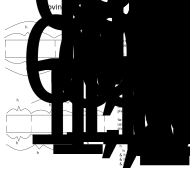
\includegraphics{merkle-equality.png}
\caption{Recursive (i.e., branch) proving cases for instances of $h_0 \equiv h_1$, meaning that $h_0$ and $h_1$ are both root hashes of Merkleizations of the same value.}
\label{fig:merkle-equality}
\end{figure}

Figure~\ref{fig:merkle-equality} depicts the recursive (i.e., branch) cases of the proof scheme for instances of $h_0 \equiv h_1$. There are two different cases to consider, distinguished by whether $h_0$ and $h_1$ have the same pivot element, or different pivot elements. A pivot element of a Merkleization with root $h$ of an object $a \in A$ is any $i \in I$ such that $h = H((h_0, h_1))$ for some $h_0, h_1$ such that $h_0$ is the root of a Merkleization of $a|_i$ and $h_1$ is the root of a Merkleization of $a|^i$. This proof scheme assumes, as previously stated, that every non-leaf Merkleization has a pivot element; such a pivot element need not be unique. To prove $h_0 \equiv h_1$ where $h_0$ and $h_1$ are roots of non-leaf Merkleizations, one can use the non-recursive case of the proof scheme (if the Merkleizations are small enough to satisfy the time and space bounds of the zk-VM), or one can use any applicable recursive case of the proof scheme. At least one of the two recursive cases will be applicable to two non-leaf Merkleizations, and in some cases both will be applicable.

To prove that $h_0 \equiv h_1$ recursively, where $h_0$ and $h_1$ are the roots of non-leaf Merkleizations of the same object, both with the same pivot element $i$, it suffices to show that there are hashes $h_{0,0},$ $h_{0,1},$ $h_{1,0}$ and $h_{1,1}$, such that:
\begin{enumerate}
\item $h_0 = H((h_{0,0}, h_{0,1}))$, that is, $h_{0,0}$ and $h_{0,1}$ are the Merkle hashes of the immediate children of the root of the object denoted by $h_0$ (with high probability, if $h_0$ is the root Merkle hash of a non-leaf object);
\item $h_1 = H((h_{1,0}, h_{1,1}))$, that is, $h_{1,0}$ and $h_{1,1}$ are the Merkle hashes of the immediate children of the root of the object denoted by $h_1$ (w.h.p., if $h_1$ is the root Merkle hash of a non-leaf object);
\item $h_{0,0} \equiv h_{1,0}$ and $h_{0,1} \equiv h_{1,1}$; that is, the left children of $h_0$ and $h_1$ are hashes denoting the same object, and the right children of $h_0$ and $h_1$ are hashes denoting the same object.
\end{enumerate}
The recursive zk-VM computation proving $h_0 \equiv h_1$, using the same pivot element $i$, directly verifies claims (1) and (2), and verifies SNARKs output by the proving process run over itself in order to probabilistically verify claims (3). 

TODO: proving scheme for equality of Merkleizations

\subsection{Set and sequence proof schemes}

The ZK proving system requires some primitives for recursively proving facts about sets and sequences. Specifically, we need to be able to prove facts of the following forms:

\begin{enumerate}
	\item For sets $A, B, C$, $A \cup B = C$.
	\item For sets $A, B$, $A \cap B = \emptyset$.
	\item For sets $A, B$ and partial computable functions $f$, $f(A) = B$.\footnote{$f(A)$ denotes the image of the set $A$ under the function $f$, i.e., $\{f(a) | a \in A\}$.}
	\item For sequences $e, e_0, e_1$, $e = e_0 \smallfrown e_1$.
\end{enumerate}

The motivation for being able to recursively prove such facts is to be able to deal with sets and sequences that are larger than what we can deal with directly in a single proof. In particular, we wish to prove statements of the following forms:

\begin{enumerate}
	\item For hashes $h, h_0, h_1$, there are sets $A, B, C$ such that $A \cup B = C$, $H(C) = h$, $H(A) = h_0$, and $H(B) = h_1$.
	\item For hashes $h_0, h_1$, there are sets $A, B$ such that $A \cap B = \emptyset$, $H(A) = h_0$, and $H(B) = h_1$.
	\item For hashes $h_0, h_1$, there are sets $A, B$ such that $f(A) = B$, $h(A) = h_0$, and $h(B) = h_1$. (This statement form is for a fixed function $f$.)
	\item For hashes $h, h_0, h_1$, there are sequences $e, e_0, e_1$ such that $e = e_0 \smallfrown e_1$, $H(e) = h$, $H(e_0) = h_0$, and $H(e_1) = h_1$.
\end{enumerate}

For each of these statement forms, there is an applicable recursive proof scheme. For each recursive proof scheme, a proof may be either a leaf or a branch proof. A leaf proof proves a statement of the specified form by proving the execution of a computation which directly verifies the statement. A branch proof verifies two or more ZK proofs of the same scheme, and verifies that the statements those inner proofs prove suffice for the truth of the statement it verifies.

Let $\uplus$ be a partial computable function of two sets and a set element, defined as follows. For interpreting applications of $\uplus$, there is implied to be a total ordering relation which applies to set elements. An application of $\uplus$ will be denoted by $A \uplus_x B$, where $A, B$ are the sets and $x$ is the set element. $x$ is called the pivot element. $A \uplus_x B$ is equal to $A \cup B$, if and only if $a \leq x$ for all $a \in A$ and $x < b$ for all $b \in B$. Otherwise, $A \uplus_x B$ is undefined.

Here is a description of the branch proofs in the set union recursive proving scheme. Suppose for given hashes $h, h_0, h_1$, we want to show there are sets $A, B, C$ such that $A \cup B = C$, $H(C) = h$, $H(A) = h_0$, and $H(B) = h_1$. We do so by proving that there are sets $A_0, A_1, B_0, B_1, C_0, C_1$ and a set element $x$ such that:
\begin{enumerate}
	\item $A_0 \uplus_x A_1 = A$.
	\item $B_0 \uplus_x B_1 = B$.
	\item $C_0 \uplus_x C_1 = C$.
	\item $A_0 \cup B_0 = C_0$.
	\item $A_1 \cup B_1 = C_1$.
\end{enumerate}
These facts suffice to imply that $A \cup B = C$. If $A \cup B = C$ and $A, B, C$ are nonempty, then such a set of facts can be constructed, and doing so suffices to reduce the problem of proving $A \cup B = C$ to two smaller set union proving problems. Those smaller set union proving problems can be proven in ZK and their proofs verified recursively.

This proving scheme for set unions requires a system for succinctly verifying facts of the form $A \uplus_x B = C$. Specifically, this can be done by succinctly verifying statements of the form: for given $h, h_0, h_1, h_x$, there are sets $A, B, C$ and a set element $x$ such that $A \uplus_x B = C$, $H(A) = h_0$, $H(B) = h_1$, $H(C) = h$, and $H(x) = h_x$. Such a statement can be verified in $O(1)$ when sets are Merkleized, because it just requires that $h$ be the root of a Merkleization of $C$ which decomposes $C$ into $A \setminus \{x\}, \{x\}$, and $B$. It should be denoted that this proving scheme does require that we can choose $h$ to be whatever the root of whatever Merkleization of $C$ makes this proving scheme work.

Here is a description of the branch proofs in the set disjointness proving scheme. Suppose for given hashes $h_0, h_1$, we want to show there are sets $A, B$ such that $A \cap B = \emptyset$, $H(A) = h_0$, and $H(B) = h_1$. We do so by proving that there are sets $A_0, A_1, B_0, B_1$ and a set element $x$ such that:
\begin{enumerate}
	\item $A_0 \uplus_x A_1 = A$.
	\item $B_0 \uplus_x B_1 = B$.
	\item $A_0 \cap B_0 = \emptyset$.
	\item $A_1 \cap B_1 = \emptyset$.
\end{enumerate}
These facts suffice to imply that $A \cap B = \emptyset$. If $A, B$ are nonempty and $A \cap B = \emptyset$, then such a set of facts can be constructed, and doing so suffices to reduce the problem of proving $A \cap B = \emptyset$ to two smaller set disjointness proving problems.

Here is a description of the branch proofs in the set image proving scheme. Suppose for given hashes $h_0, h_1$, we want to show there are sets $A, B$ such that $f(A) = B$, $H(A) = h_0$, and $H(B) = h_1$. We do so by proving that there are sets $A_0, A_1, B_0, B_1$ and a set element $x$ such that:
\begin{enumerate}
	\item $A_0 \uplus_x A_1 = A$.
	\item $B_0 \uplus_x B_1 = B$.
	\item $f(A_0) = B_0$.
	\item $f(A_1) = B_1$.
	\item $B_0 \cup B_1 = B$.
\end{enumerate}
These facts suffice to imply that $f(A) = B$. If $A$ is nonempty and $f(A) = B$, then such a set of facts can be constructed, and doing so suffices to reduce the problem of proving $f(A) = B$ to two smaller set image proving problems.

The sequence concatenation proving scheme wants to show, for given $h, h_0, h_1$, that there are sequences $e, e_0, e_1$ such that $e = e_0 \smallfrown e_1$, $H(e) = h$, $H(e_0) = h_0$, and $H(e_1) = h_1$. It works by Merkleizing $e$ in such a fashion that $h = H((h_0, h_1))$. This scheme requires being able to choose $h$ to be the one that makes this scheme work, out of all of the different ways of Merkleizing $e$.

\section{Application proof schemes}

The ZK proving system needs to prove statements of the following forms. For each of these forms, the instance data consists of the hash $h$.

\begin{enumerate}
	\item There is a $t \in T$ such that $H(t) = h$ and $\text{coherent}(t) = 1$.
	\item There is $x \in T \times C$ such that $H(x) = h$ and $\text{applies}(t, c) = 1$.
	\item There is $x = (t, c, s) \in T \times C \times E$ such that $H(x) = h$ and $\text{schedule}(t, c) = s$.
	\item There is $x = (t, c_0, e, c_1) \in T \times C \times E \times C$ such that $H(x) = h$ and $\text{update}(t, c_0, e) = c_1$.
\end{enumerate}

For each of these statement forms, there is an applicable recursive proof scheme. The reason for the proof schemes being recursive is that we assume that there is an upper bound on the amount of computation we can verify in a single proof, but we require the system to scale to function executions on arbitrarily complex inputs. For each recursive proof scheme, a proof may be either a leaf or a branch proof. A leaf proof proves a statement of the specified form by directly proving the evaluation of the function on the given input. A branch proof verifies two or more ZK proofs of the same scheme, and verifies that the statements those inner proofs prove suffice for the truth of the statement it verifies.

Although branch proofs are described below with exactly two children, the descriptions can be extended in a straightforward manner to allow for branching factors greater than two.

A branch proof of $\text{coherent}(t) = 1$ verifies that there are some $t_0, t_1 \in T$ such that $t_0 \vee t_1 = t$, $\text{coherent}(t_0) = 1$, $\text{coherent}(t_1) = 1$, and $\text{id}(t_0) \cap \text{id}(t_1) = \emptyset$. The instance data in this case is $H((h_0, h_1))$, where $h_i$ is the Merkleization of $t_i$. This proving scheme makes use of the proving schemes for set union (to prove $t_0 \vee t_1 = t$), set image under id (to prove the values of $\text{id}(t_0)$ and $\text{id}(t_0)$), and set disjointness (to prove $\text{id}(t_0) \cap \text{id}(t_1) = \emptyset$).

A branch proof of $\text{applies}(t, c) = 1$ verifies that there are some $t_0, t_1 \in T$ and $c_0, c_1 \in C$ such that $t_0 \vee t_1 = t$, $\text{id}(t_0) \cap \text{id}(t_1) = \emptyset$, and $c_0 \oplus c_1 = c$, such that $\text{applies}(t_0, c_0) = 1$, and $\text{applies}(t_1, c_1) = 1$. The instance data in this case is $H((h_0, h_1))$, where $h_i$ is the Merkleization of $(t_i, c_i)$. This proving scheme makes use of the proving schemes for set union (to prove $t_0 \vee t_1 = t$), set image under id (to prove the values of $\text{id}(t_0)$ and $\text{id}(t_1)$), and set disjointness (to prove $\text{id}(t_0) \cap \text{id}(t_1) = \emptyset$). This proving scheme also requires a proving scheme for proving instances of $c = c_0 \oplus c_1$.

Next, let's look at a recursive proving scheme for proving instances of $c = c_0 \oplus c_1$, for $c, c_0, c_1 \in C$. Specifically, this scheme will prove statements of the following form. For given $h, h_0, h_1$, there are $c, c_0, c_1 \in C$ such that $c = c_0 \oplus c_1$, $H(c) = h$, $H(c_0) = h_0$, and $H(c_1) = h_1$.

Recall that for $c = c_0 \oplus c_1$ to be true, the following conditions are necessary and sufficient: there are $t_0, t_1 \in T$ such that $\text{applies}(t_0, c_0) = 1$, $\text{applies}(t_1, c_1) = 1$, $t_0 \wedge t_1 = \emptyset_T$, and $\text{asOf}(c_0) = \text{asOf}(c_1)$. The statement $\text{asOf}(c_0) = \text{asOf}(c_1)$ is assumed to be directly verifiable in $O(1)$, by opening the Merkleizations of $c_0$ and $c_1$ to a constant depth to read the value of a timestamp field on the structures. The other elements of the conditions for $c = c_0 \oplus c_1$ can be proven and succinctly verified using methods already defined.

There is a circularity in the definitions of the recursive proving schemes for applies and $\oplus$, since each references the other. This is okay, because the proving scheme for each one references the proving scheme for the other one with respect to smaller subproblems only; so it does not lead to an infinite regress.

For branch (i.e., recursive) proofs of instances of $\text{update}(t, c_0, e) = c_1$, there are two kinds: the vertically sliced and horizontally sliced kinds. The vertically sliced kind decompose the problem into smaller subproblems by reducing the number of contracts involved. The horizontally sliced kind decompose the problem into smaller subproblems by reducing the number of events involved.

A \emph{vertically sliced}\/ branch proof of $\text{update}(t, c_0, e) = c_1$ verifies that there are some $t_0, t_1 \in T$ and $c_{0,0}, c_{0,1}, c_{1,0}, c_{1,1} \in C$ such that $t_0 \vee t_1 = t$, $\text{id}(t_0) \cap \text{id}(t_1) = \emptyset$, $c_{0,0} \oplus c_{0,1} = c_0$, $c_{1,0} \oplus c_{1,1} = c_1$, $\text{update}(t_0, c_{0,0}, e) = c_{1,0}$, and $\text{update}(t_1, c_{0,1}, e) = c_{1,1}$. The instance data in this case is $H((h_0, h_1))$, where $h_i$ is the Merkleization of $(t_i, c_{0,i}, e, c_{1,i})$. This proving scheme makes use of the proving schemes for set union (to prove $t_0 \vee t_1 = t$), set image under id (to prove the values of $\text{id}(t_0)$ and $\text{id}(t_1)$), and set disjointness (to prove $\text{id}(t_0) \cap \text{id}(t_1) = \emptyset$). It also makes use of the $\oplus$ proving scheme.

A \emph{horizontally sliced}\/ branch proof of $\text{update}(t, c_0, e) = c_2$ verifies that there are some $e_0, e_1 \in E$ and $c_1 \in C$ such that $e = e_0 \smallfrown e_1$, and $\text{update}(t, c_0, e_0) = c_1$, and $\text{update}(t, c_1, e_1) = c_2$. The instance data in this case is $H((h_0, h_1))$, where $h_i$ is the Merkleization of $(t, c_i, e_i, c_{1+i})$. This proving scheme makes use of the sequence concatenation proving scheme.

Finally, let's look at a recursive proving scheme for proving instances of $\text{schedule}(t, c) = e$. Specifically, this scheme will prove statements of the following form. For given $h_i, h_o$, there are $t \in T$, $c \in C$, and $e \in E$ such that $H((t, c)) = h_i$, $H(e) = h_o$, and $\text{schedule}(t, c) = e$.

The branch proofs decompose the problem into smaller subproblems by splitting up the $T$ elements and $C$ elements, taking advantage of the homomorphic property of the scheduling function, that is (with suppressed premises):
\begin{equation}
\text{schedule}(t_0, c_0) \vee \text{schedule}(t_1, c_1) = \text{schedule}(t_0 \vee t_1, c_0 \oplus c_1).
\end{equation}
A branch scheduling proof verifies, for given hashes $h_i, h_o$, that there are $t, t_0, t_1 \in T$, $c, c_0, c_1 \in C$, and $e, e_0, e_1 \in E$, such that $\text{applies}(t_0, c_0) = 1$, $\text{applies}(t_1, c_1) = 1$, $t_0 \vee t_1 = t$, $c_0 \oplus c_1 = c$, $e_0 \vee e_1 = e$, $H((t, c)) = h_i$, and $H(e) = h_o$. It verifies these facts indirectly by verifying that there are hashes $h_{i,0}, h_{i,1}, h_{o,0}, h_{o,1}$ such that:
\begin{enumerate}
\item $h_i = H((h_{i,0}, h_{i,1}))$.
\item $h_o = H((h_{o,0}, h_{o,1}))$.
\item For each $k \in \{0,1\}$, $h_{i,k}$ is the root of a Merkleization of a pair $(t_k, c_k) \in T \times C$, and $h_{o,k}$ is the root of a Merkleization of an event sequence $e_k \in E$, such that:
	\begin{enumerate}
	\item $\text{applies}(t_k, c_k) = 1$, for each $k \in \{0,1\}$.
	\item $\text{schedule}(t_k, c_k) = e_k$, for each $k \in \{0,1\}$.
	\item $\text{id}(t_0) \cap \text{id}(t_1) = \emptyset$.
	\item $e_0 \wedge e_1 = e$.
	\end{enumerate}
\end{enumerate}
These facts suffice to imply the given instance. All of these facts can be proven by methods already outlined, except for $e_0 \wedge e_1 = e$, which requires a method for proving unions of event sequences. Such a method should be easy enough to devise by following the example of the set union proving scheme.

\section{Future directions}

Can we be more intelligent about considering which events matter for which contracts? Currently the best possible worst case proving complexity of this scheme is $O(n \times m)$ in $n$ the number of contracts and $m$ the number of events. For global events, such as interest rate changes, this may be the best possible worst case proving complexity, because if $O(n)$ contracts are impacted by an event then $O(n)$ many contract schedules need to be recomputed upon such an event. However, plausibly, most events impact only a small number of contracts, typically only a single one. The proving scheme could be refined to allow for events that impact a limited subset of contracts to be run over only a subset of all contracts containing the impacted subset.

\end{document}
